

%=================================================================
% Outline
%=================================================================
%\section{Introduction}
%% Auto-generate the TOC slide(s)
\begin{frame}
  \tableofcontents[currentsection]
  %\tableofcontents
\end{frame}

\section*{Outline}% Make it easy to jump to this page in the PDF

% Auto-generate the TOC slide(s)
\begin{frame}
  \frametitle{Outline}
  %\tableofcontents[currentsection]
  \tableofcontents
\end{frame}




\section{Introduction}
%%%%%%%%%%%%%%%%%%%%%%%%%%%%%%%%%%%%%%%%%%%%%%%%%
\frame
{
  \frametitle{Background}

  \begin{itemize}
  \item Modern simulation software is \emphcolor{complex}:
    \begin{itemize}
    \item Implicit numerical methods
    \item Massively parallel computers
    \item Adaptive methods
    \item Multiple, coupled physical processes
    \end{itemize}
    %\pause
  \item There are a host of existing software libraries that excel at treating various aspects of this complexity.
  \item Leveraging existing software whenever possible is the most efficient way to manage this complexity.

  \end{itemize}
}




%%%%%%%%%%%%%%%%%%%%%%%%%%%%%%%%%%%%%%%%%%%%%%%%%
\frame
{
  \frametitle{Background}

  \begin{itemize}
  \item Modern simulation software is \emphcolor{multidisciplinary}:
    \begin{itemize}
    \item Physical Sciences
    \item Engineering
    \item Computer Science
    \item Applied Mathematics
    \item \ldots
    \end{itemize}
  \item It is not reasonable to expect a single person to have all the necessary skills for developing \& implementing high-performance numerical algorithms on modern computing architectures.
  \item Teaming is a prerequisite for success.
  \end{itemize}
}


 

%%%%%%%%%%%%%%%%%%%%%%%%%%%%%%%%%%%%%%%%%%%%%%%%%
\frame
{
  \frametitle{Background}                 
  \begin{itemize}
    \item A large class of problems are amenable to \emphcolor{mesh based} simulation techniques.
      %% \begin{columns}[t]
      %%   \column{.5\textwidth}        
      %%   \fbox{\includegraphics[viewport=140 420 400 685,clip=true,height=1in]{domain2/domain2_input}}
      %%   \column{.5\textwidth}
      %%   \fbox{\includegraphics[height=1in,angle=-90]{discretized_domain}}
      %% \end{columns}
    \item Consider some of the major components such a simulation:
      \pause
      \begin{enumerate}
        \item Read the mesh from file
        \item Initialize data structures
        \item Construct a discrete representation of the governing equations
        \item Solve the discrete system
        \item Write out results
        \item Optionally estimate error, refine the mesh, and repeat
      \end{enumerate}

    \pause
    \item With the exception of step 3, the rest is \emph{independent} of the class of problems being solved.
    \pause
    \item This allows the major components of such a simulation to be abstracted \& implemented in a reusable software library.
  \end{itemize}
}


 

\subsection{The \libmesh{} Software Library}
%%%%%%%%%%%%%%%%%%%%%%%%%%%%%%%%%%%%%%%%%%%%%%%%%
\frame
{
  \frametitle{The \libmesh{} Software Library}
  \begin{itemize}
    \item In 2002, the \libmesh{} library began with these ideas in mind.
    \item Primary goal is to provide data structures and algorithms that can be shared by disparate physical applications, that may need some combination of
      \begin{itemize}
      \item Implicit numerical methods
      \item Adaptive mesh refinement techniques
      \item Parallel computing
      \end{itemize}
    \item Unifying theme: \emphcolor{mesh-based simulation of partial differential equations (PDEs)}.
  \end{itemize}
}



 

\subsection{Software Reusability}
%%%%%%%%%%%%%%%%%%%%%%%%%%%%%%%%%%%%%%%%%%%%%%%%%
\frame
{
  \frametitle{The \libmesh{} Software Library}

  \begin{block}{Key Point}
    \begin{itemize}
      \item The \libmesh{} library is designed to be used by students, researchers, scientists, and engineers as a tool for \emphcolor{developing simulation codes} or as a tool for \emphcolor{rapidly implementing a numerical method}.
      \item \libMesh{} is not an application code.
      \item It does not ``solve problem XYZ.''
        \begin{itemize}
          \item It can be used to help you develop an application to solve problem XYZ, and to do so quickly with advanced numerical algorithms on high-performance computing platforms.
        \end{itemize}
      %\item It was initially targeted for finite element based simulations, but has been used for finite volume discretizations as well.
    \end{itemize}    
  \end{block}
} 


\begin{frame}{libMesh Community}
\begin{columns}
\column{.4\textwidth}
\begin{block}{Scope}
\begin{itemize}
\item Free, Open source
\begin{itemize}
\item LGPL2 for core
\end{itemize}
\item 35 Ph.D.\ theses, 393 papers (58 in 2015)
\item $\sim10$ current developers
\item $160-240$ current users?
\end{itemize}
\end{block}

\column{.6\textwidth}
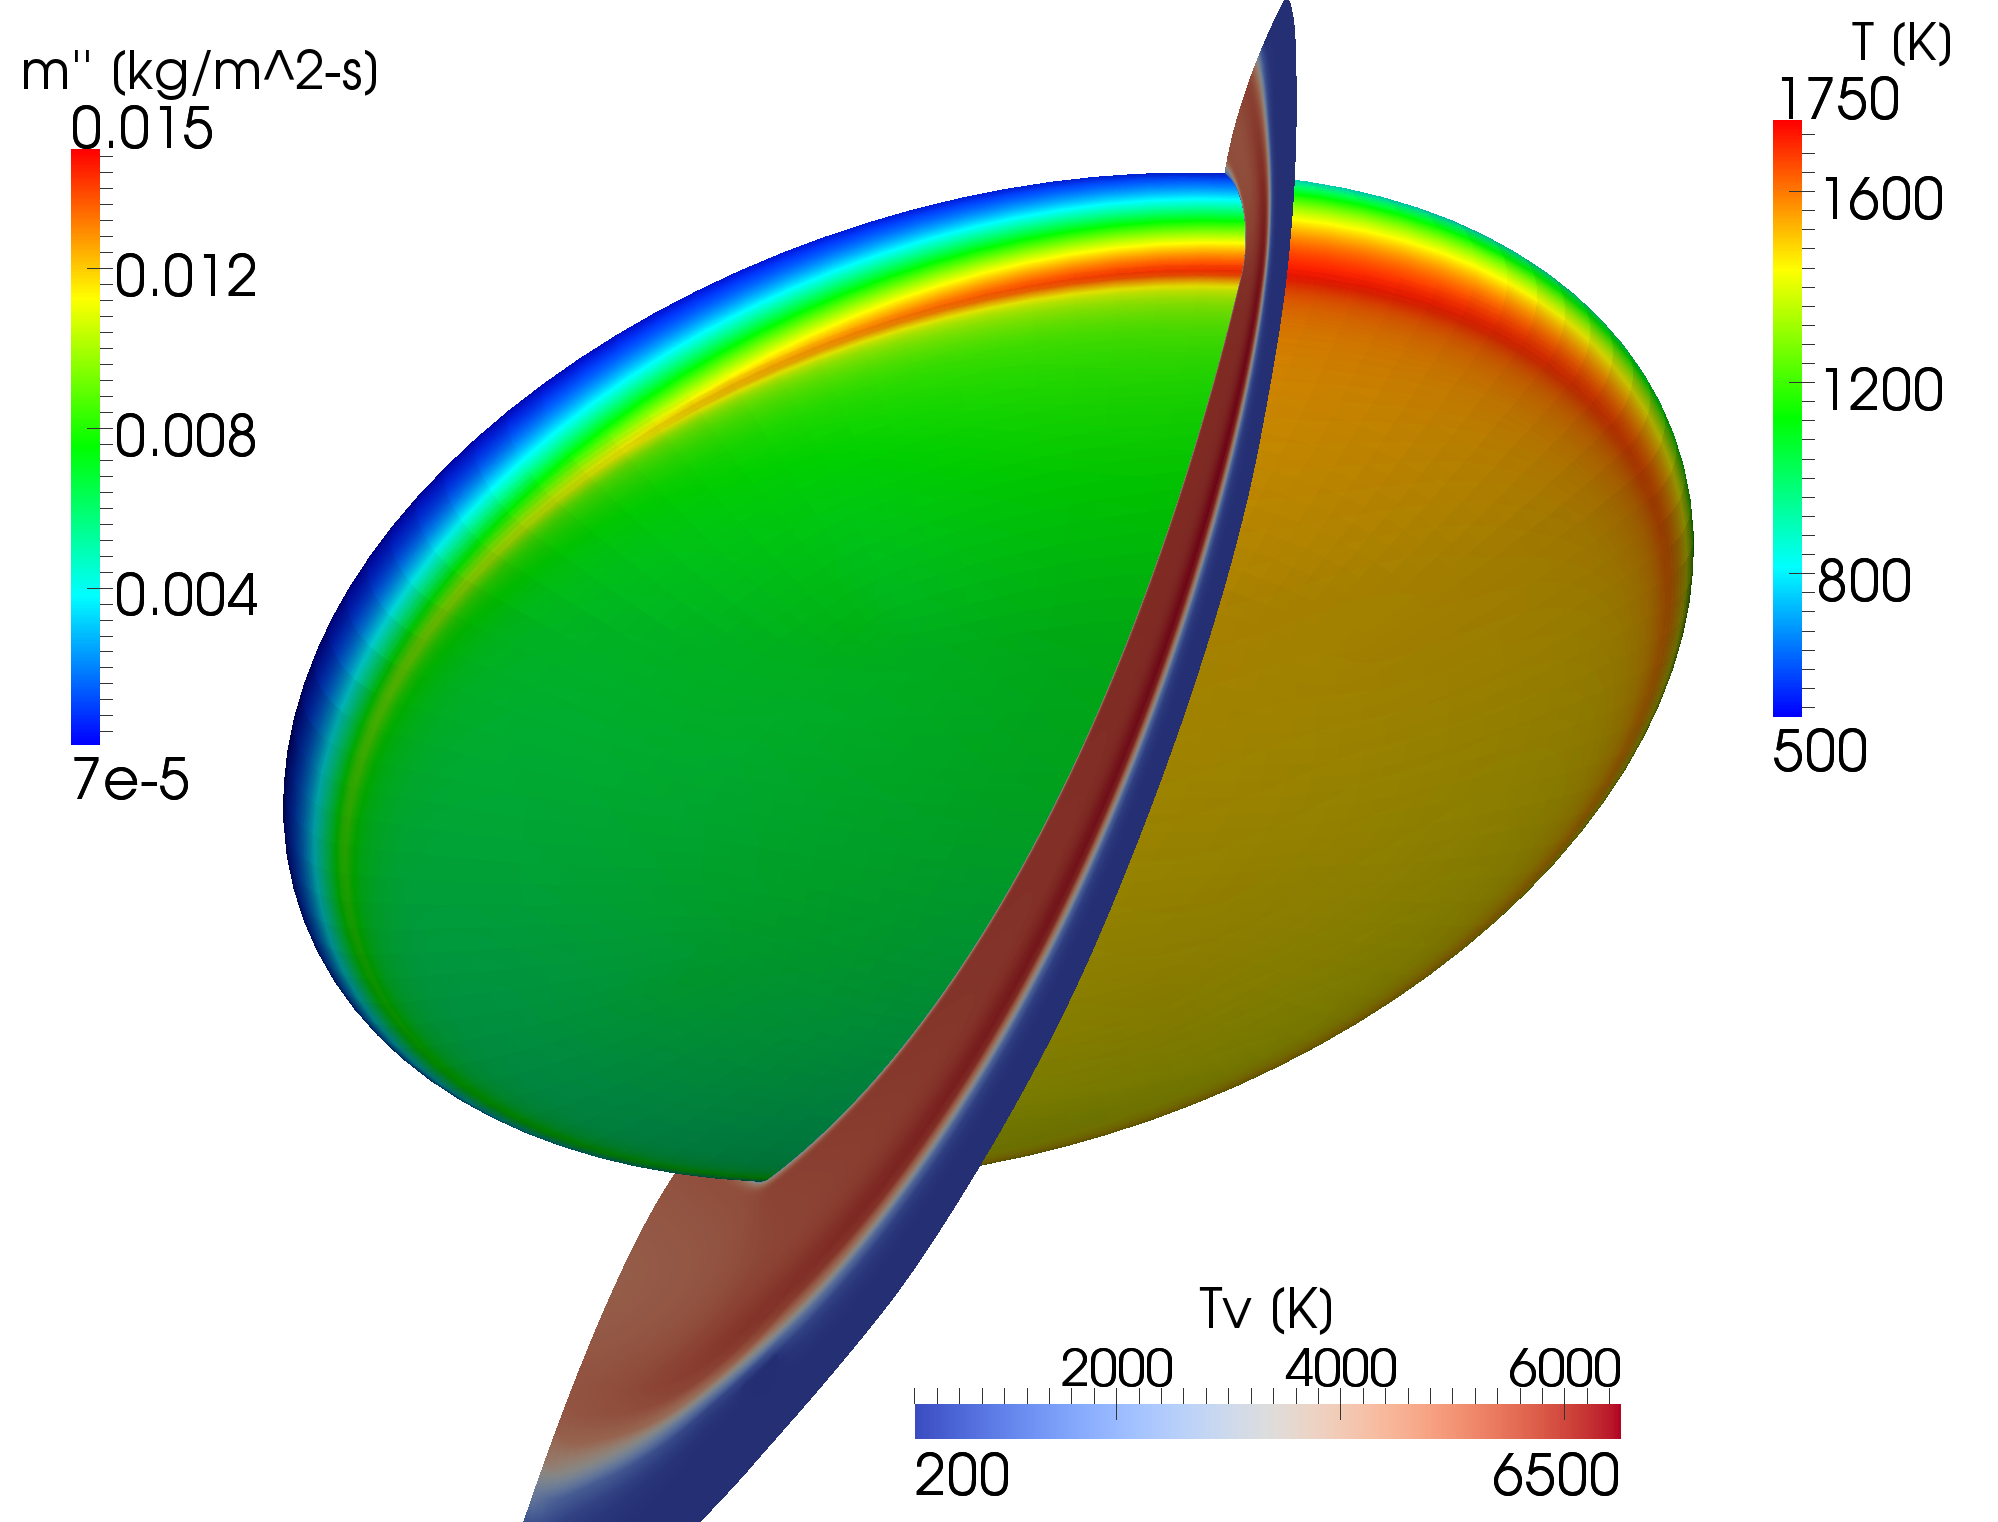
\includegraphics[width=.45\textwidth]{ablating_hs_wbg}
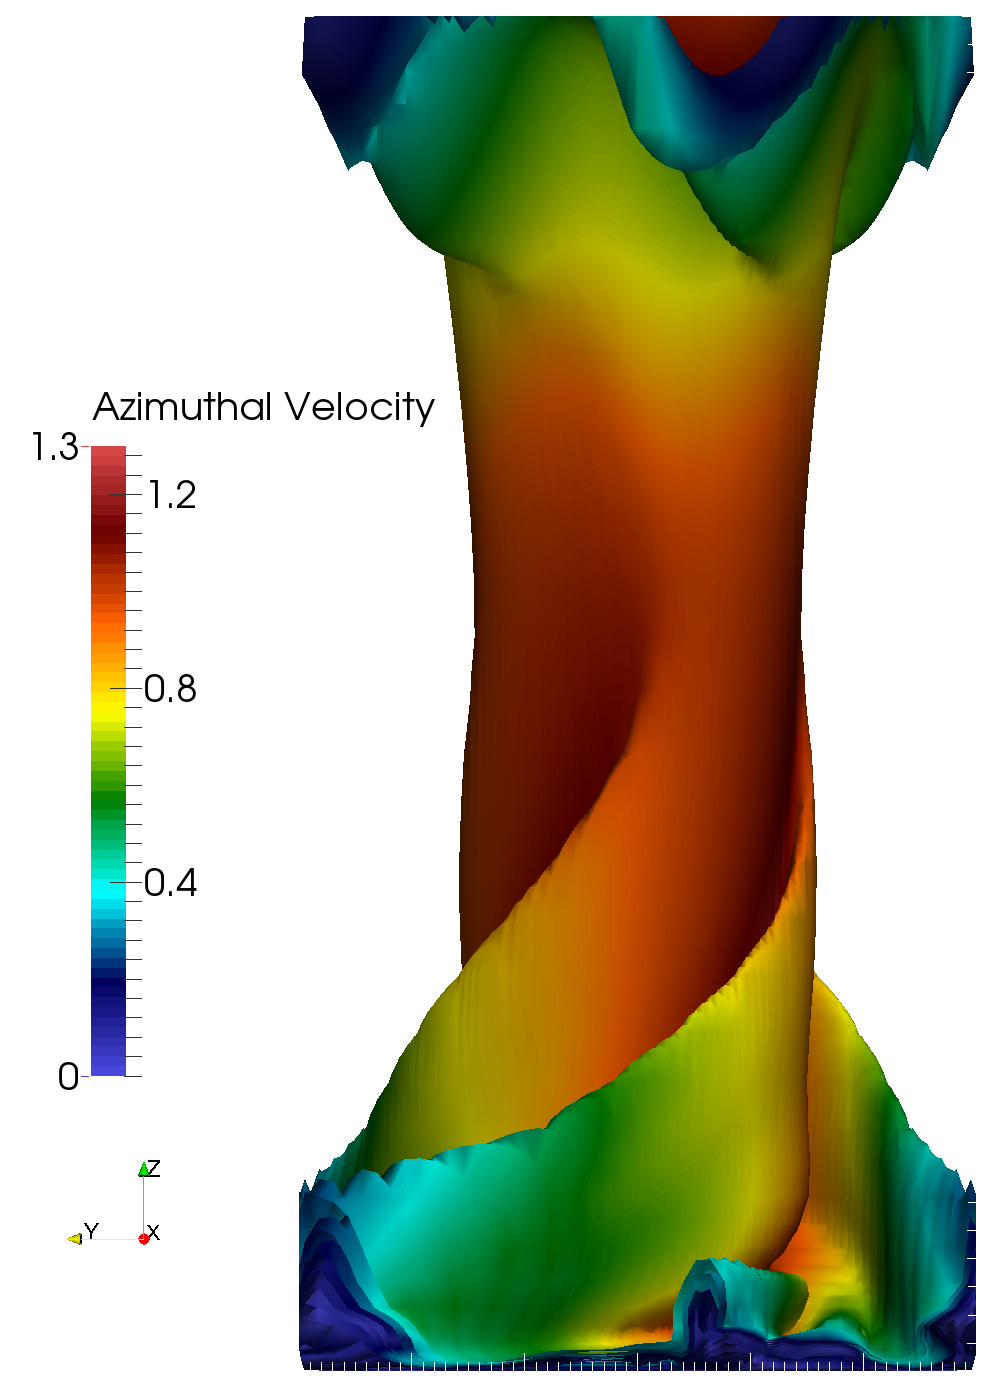
\includegraphics[width=.25\textwidth]{sov}
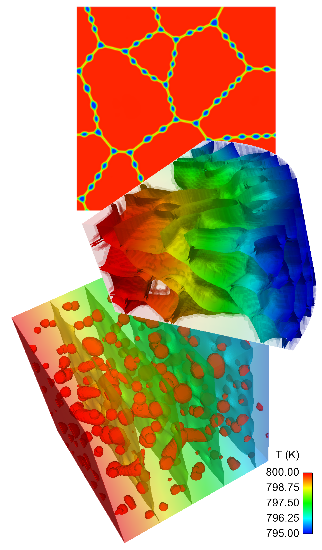
\includegraphics[width=.3\textwidth]{marmot1b}
\end{columns}

\begin{columns}
\column{.35\textwidth}
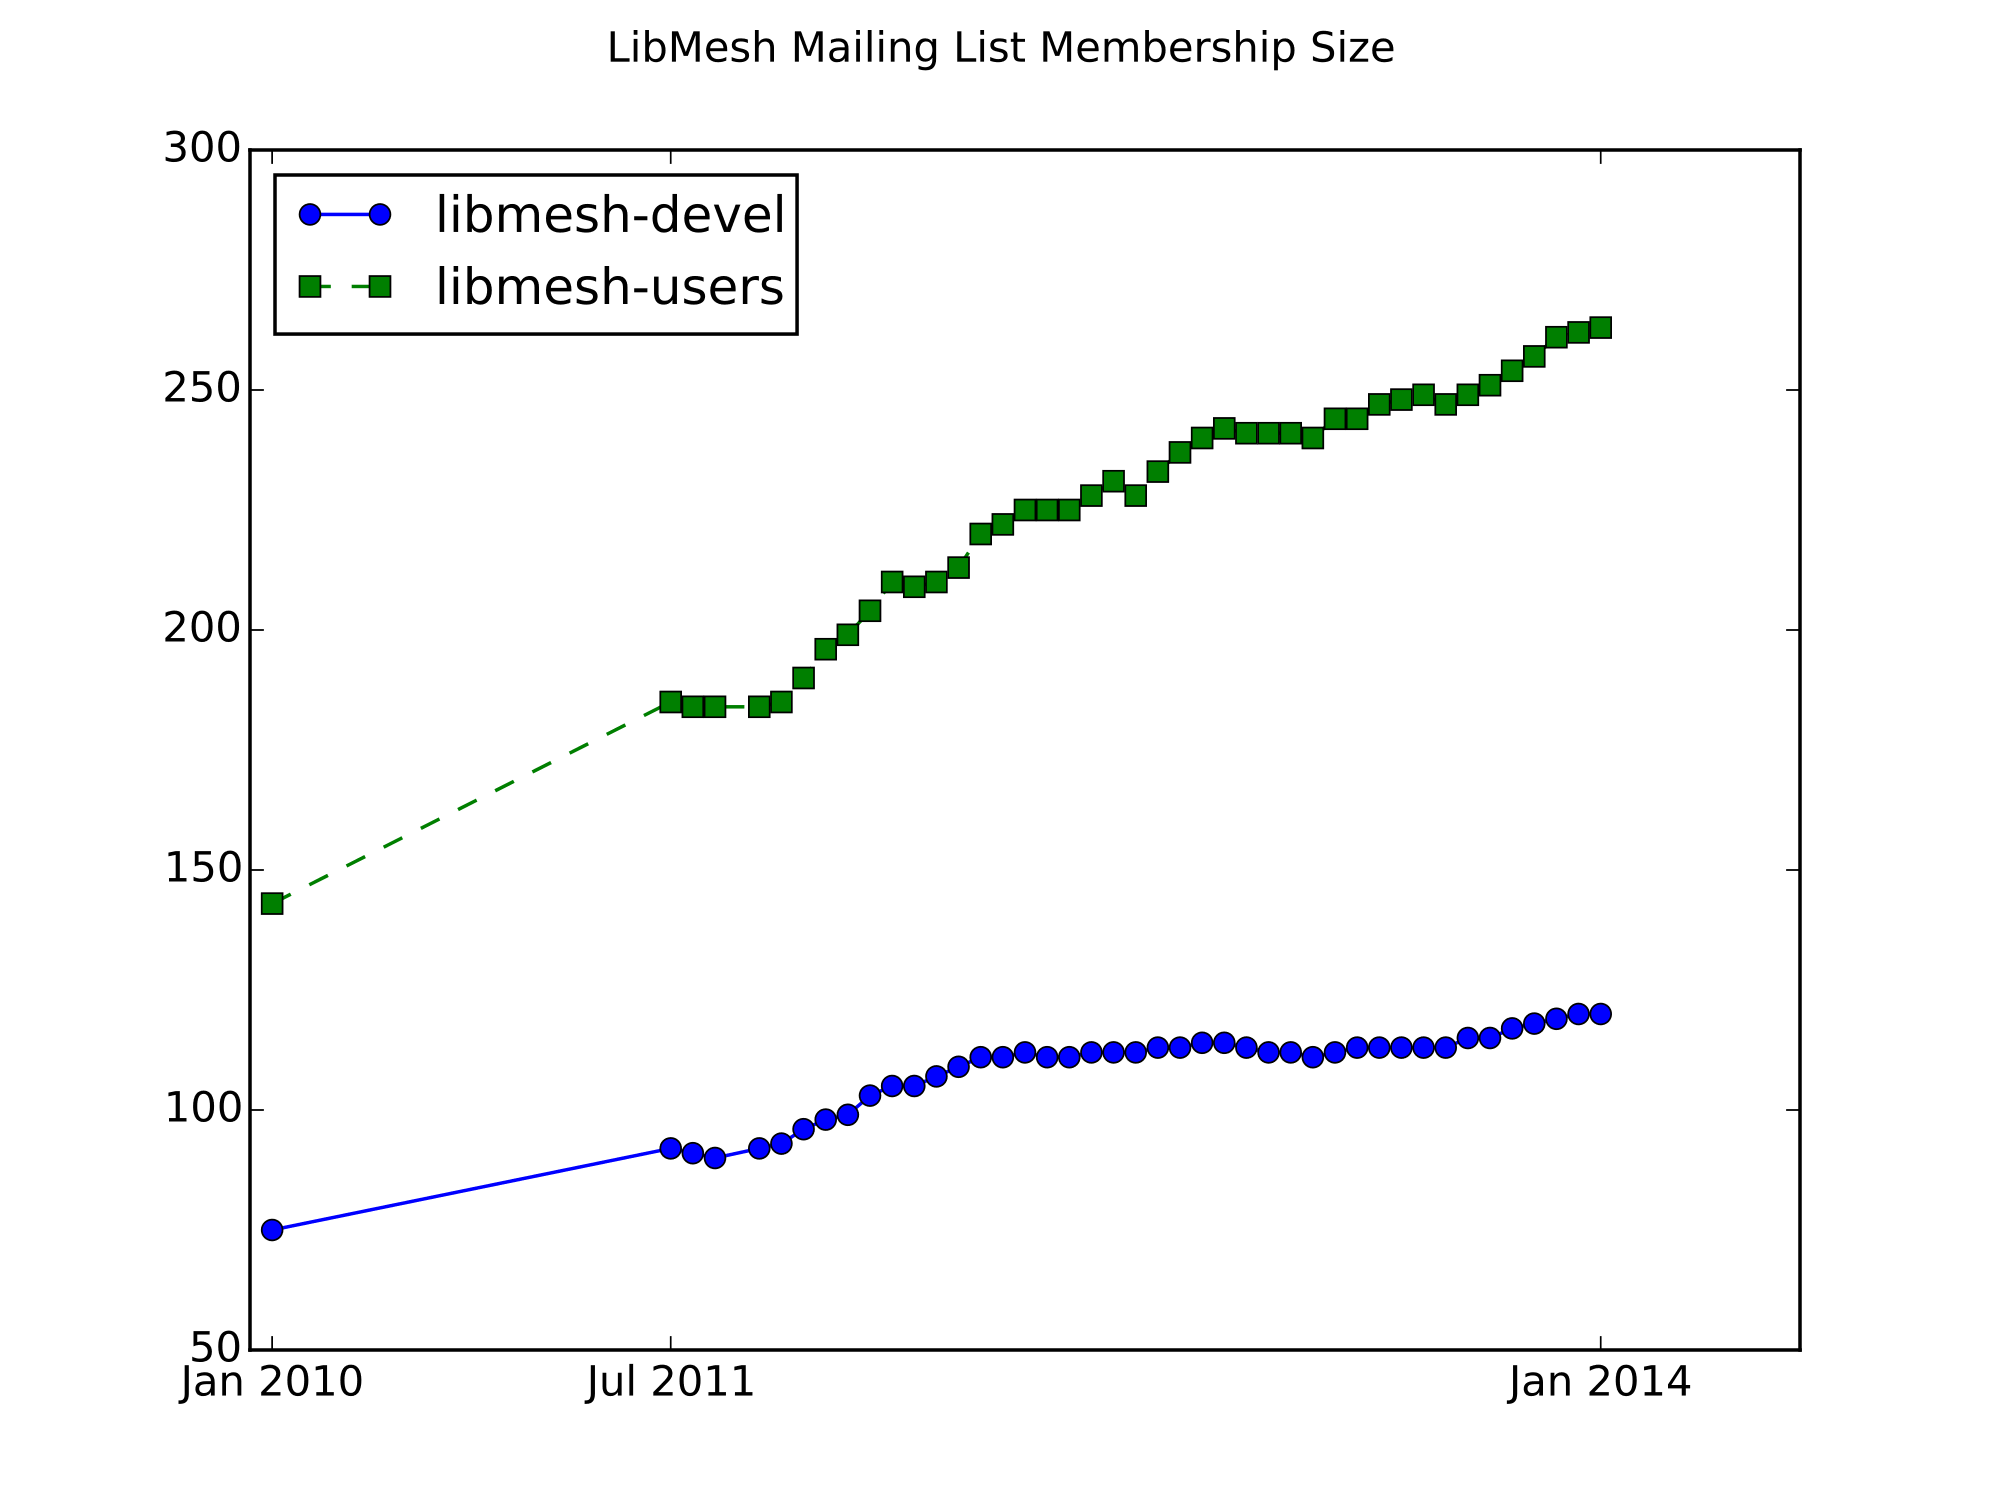
\includegraphics[width=\textwidth]{libmesh_mailinglists_membership}

\column{.65\textwidth}
\begin{block}{Challenges}
\begin{itemize}
\item Radically different application types
\item Widely dispersed core developers
\begin{itemize}
\item INL, UT-Austin, U.Buffalo, JSC, MIT, Harvard, Argonne
\end{itemize}
\item OSS, commercial, private applications
\end{itemize}
\end{block}
\end{columns}

\end{frame}


\begin{frame}[t]
  \begin{columns}
    \column{.6\textwidth}
    \begin{center}
      \includegraphics[width=.9\textwidth]{mytreeandroots_allnames}
    \end{center}
    \column{.35\textwidth}
    \begin{itemize}
      \item Foundational (typically optional) library access via LibMesh's ``roots''.
      \item Application ``branches'' built off the library ``trunk''.
      \item Additional middleware layers (e.g. Akselos, GRINS, MOOSE) for more complex applications
    \end{itemize}
  \end{columns}

\end{frame}




%%%%%%%%%%%%%%%%%%%%%%%%%%%%%%%%%%%%%%%%%%%%%%%%%
\frame
{
  \frametitle{Software Reusability}
  \begin{itemize}
    \item At the inception of \libMesh{} in 2002, there were many high-quality software libraries that implemented some aspect of the end-to-end PDE simulation process:
      \begin{itemize}
        \item Parallel linear algebra
        \item Partitioning algorithms for domain decomposition
        \item Visualization formats
        \item \ldots
      \end{itemize}
    \item A design goal of \libMesh{} has always been to provide flexible \& extensible interfaces to existing software whenever possible.
    \item We implement the ``glue'' to these pieces, as well as what we viewed as the missing infrastructure:
      \begin{itemize}
        \item \emphcolor{Flexible data structures for the discretization of spatial domains and systems of PDEs posed on these domains.}
      \end{itemize}          
  \end{itemize}  
}


\section{Library Design}


\begin{frame}
\frametitle{Geometric Element Classes}

\begin{columns}
\column{.55\textwidth}
\begin{center}
\vspace{-5mm}
\includegraphics[width=.75\textwidth]{DofObjects}
\end{center}
\column{.45\textwidth}
\begin{itemize}
\item Abstract interface gives mesh topology
\item Concrete instantiations of mesh geometry
\item Hides element type from most applications
\item Runtime polymorphism allows mixed element types, dimensions
\item Base class data arrays allow more optimization, inlining
\end{itemize}

\end{columns}

\end{frame}


%%%%%%%%%%%%%%%%%%%%%%%%%%%%%%%%%%%%%%%%%%%%%%%%%
\frame
{
  \frametitle{Linear Algebra}
  \begin{center}
    \includegraphics[width=\textwidth,trim=7.56in 0 0 0,clip]{libmesh_docs/classlibMesh_1_1SparseMatrix__inherit__graph}
  \end{center}
}



%%%%%%%%%%%%%%%%%%%%%%%%%%%%%%%%%%%%%%%%%%%%%%%%%
\frame
{
  \frametitle{I/O formats}
  \begin{center}
    \includegraphics[height=0.9\textheight]{libmesh_docs/mesh_io}
  \end{center}
}


%%%%%%%%%%%%%%%%%%%%%%%%%%%%%%%%%%%%%%%%%%%%%%%%%
\frame
{
  \frametitle{Domain Partitioning}
  \begin{center}
    \includegraphics[width=.3\textwidth]{part_trans}
    %\\
    \includegraphics[width=.3\textwidth]{streamtraces}
  \end{center}  

  \includegraphics[width=.65\textwidth]{libmesh_docs/partitioner}
}


\begin{frame}
\frametitle{Mesh Data Structures}
\begin{columns}
\column{.6\textwidth}
\begin{center}
\includegraphics[width=.95\textwidth]{MeshUML}
\end{center}
\column{.4\textwidth}
%\begin{block}{}
\begin{itemize}
\item \texttt{MeshBase} gives node or element iterators, all or active, global or local
\item \texttt{SerialMesh} or \texttt{ParallelMesh} manages synchronized or distributed data
\end{itemize}

\includegraphics[width=.75\textwidth]{ParallelMesh3}
%\end{block}
\end{columns}

\end{frame}



%%%%%%%%%%%%%%%%%%%%%%%%%%%%%%%%%%%%%%%%%%%%%%%%%
\frame
{
  \frametitle{Discretization: Finite Elements}
  \begin{center}
    \includegraphics[width=0.9\textwidth,trim=7.4in 0 0 0,clip]{libmesh_docs/classlibMesh_1_1FEAbstract__inherit__graph}
  \end{center}
}      



%%%%%%%%%%%%%%%%%%%%%%%%%%%%%%%%%%%%%%%%%%%%%%%%%
\frame
{
  \frametitle{Algorithms: Error Estimation}
  \begin{center}
    \includegraphics[width=\textwidth]{libmesh_docs/error_estimation}
  \end{center}
}





% LocalWords:  nasablue
